\section{Amélioration du prefetch de Blue Banana}

L'objectif  est de précharger plus finement les données que dans la solution introduite dans Blue Banana, et surtout d'essayer de ne pas précharger des données inutiles. Pour le moment, nous regardons juste les nœuds qui sont dans notre champs de vision (un cône) et qui ne sont ni trop loin, ni trop près. Mais il serait intéressant d'avoir plus d'informations sur les nœuds avant de les précharger, comme leur direction ou leur vitesse par exemple. Nous avons donc regardé quelques critères qui pourraient permettre de rapatrier les données de façon plus fine.

\subsection{Les changements introduits sur la version de Blue Banana}


\par Actuellement un nœud, qui est dans l'état \textbf{T}(ravelling), va chercher des nœuds qui se trouvent sur la trajectoire probable de l'avatar, tant que son ensemble de voisins n'est pas plein. Ce mécanisme va donc précharger des données qui sont à bonne distance (pas trop près à cause des temps de communication). Un des risques est de précharger des nœuds qui sont inutiles si l'avatar, dont nous préchargions les données, change de direction ou d'état. Un autre problème est que l'on peut précharger des avatars qui sont dans le cône mais qui s'en écartent ou des avatars qui arrivent à grande vitesse vers notre avatar (voir figure~\ref{prefetchav}). Le mécanisme existant n'observe pas les différentes propriétés des nœuds (vitesse, direction, état, etc). Des nœuds probablement superflus vont être rapatriés: modifier le préchargement des données pourrait nous permettre de faire ce traitement plus finement.

\par  Nous pouvons voir un exemple des modifications qu'entraineraient le nouveau préchargement, dans le schéma de la figure~\ref{prefetchav}. Les nœuds verts représentent les nœuds qui seront préchargés, les nœuds rouges ceux qui sont dans la zone de rapatriement mais qui ne le seront pas. Sur la figure, nous pouvons voir que nous gardons les nœuds qui sont stables, qui bougent peu ou qui bougent dans le même sens que le nœud courant (nœud gris foncé). Les nœud qui sont rouges ont des directions inverses au nœud courant et des vitesses élevées, ils ne seront donc pas préchargés.

	\begin{figure}[!h]
        \centering
        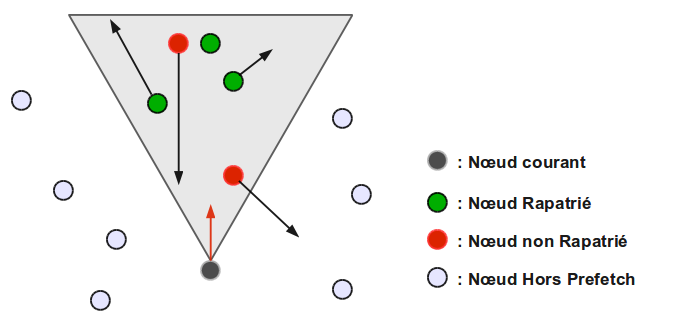
\includegraphics[scale=0.45]{./Ressources/Images/prefetchaV1.png}
        \caption{Exemple de gain possible pour le prefetching}
        \label{prefetchav}
        \end{figure}

\par Pour réaliser cette sélection, il faut donc, en plus de la distance avec le nœud, tester différentes autres propriétés. Dans les messages de préchargement actuels, se trouve le vecteur du nœud faisant la requête de préchargement. Nous pourrons, avec celui-ci, regarder la direction et la longueur de ce nœud. Nous pourrons ainsi comparer ces critères chez le nœud faisant la requête et le nœud qui a reçu le message. Une des méthodes de choix des nœuds est de sélectionner les nœuds qui sont dans l'état \textbf{T}(ravelling), en faisant la somme des normes du vecteur de préchargement et du nœud courant. Si la somme est plus grande que la norme du vecteur de préchargement, nous sélectionnons ce nœud et faisons le traitement correspondant. Cette solution laisse passer des problèmes que nous souhaitions éviter et va supprimer le rapatriement de nœud qui aurait pu être intéressant. Ainsi un nœud qui avance de façon très lente vers le nœud de prefetch ne serait pas pris car la norme serait plus petite. Ce cas peut être en partie réglé par la mise en place d'une longueur de battement.
\newline
$$\\\textit{Somme des normes des vecteurs~$\ge$~Norme du vecteur de prefetch +/- $\Delta$}$$
\\Les problèmes d'un nœud qui arrive à grande vitesse vers le nœud de préchargement ou d'un nœud qui a une direction qui s'écarte du nœud de préchargement, restent toujours en partie présents malgré la mise en place de la dernière solution. Nous avons donc cherché à regarder en plus des normes, les directions des différents nœuds et de les comparer.
\par En utilisant les directions, une des idées a été de précharger de préférence les nœuds qui vont dans la même direction (vois figure~\ref{PrefetchSol}). Si les nœuds vont vers les cotés, par rapport au vecteur de préchargement, il faut que la longueur du vecteur soit alors pas trop grande pour qu'il soit sélectionné. De même pour les nœuds qui vont dans la direction opposée au vecteur de préchargement.

%	\begin{figure}[!h]
 %       \centering
  %      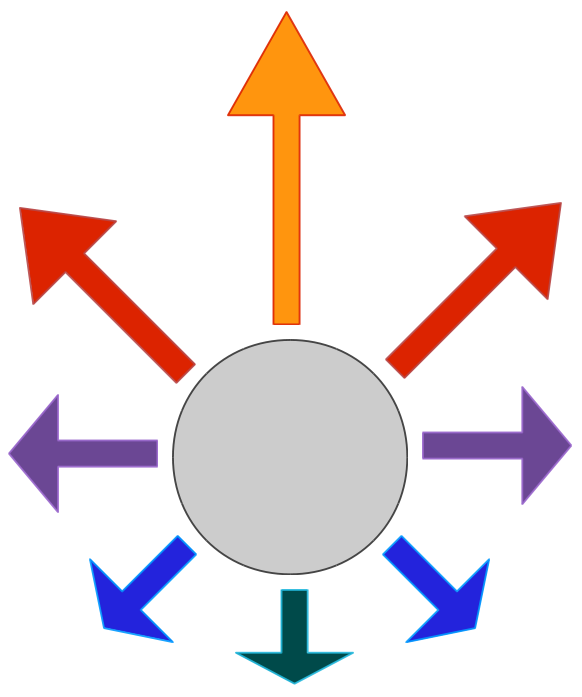
\includegraphics[scale=0.30]{./Ressources/Images/prefetchSol.png}
   %     \caption{Préférence de prefetching}
    %    \label{PrefetchSol}
     %   \end{figure}

\par Les ajouts ont été faits dans le module de mise en place du préchargement de Blue Banana. Des fonctions de comparaison d'angle et de norme y ont été ajoutées, et nous les avons insérées dans la fonction \textit{processPrefetchMsg} (voir code ci-dessous). Après avoir fait les traitements de base, comme vérifier que le nœud soit assez loin, nous testons pour savoir si le préchargement amélioré est activé. 
\newline
\\ Nous rapatrions alors les nœuds si:
        \begin{itemize}
        \renewcommand{\labelitemi}{$\bullet$}
                \item L'angle du vecteur du nœud courant est proche de l'angle du vecteur de préchargement (environ 45° de chaque côté).
		\item La somme des normes des vecteurs est supérieure la norme du vecteur de préchargement multipliée par un et demi. 
                \item Le nœud courant n'est pas dans l'état \textbf{T}(ravelling).
		\item L'angle du vecteur du nœud courant n'est pas proche de l'angle du vecteur du nœud de préchargement mais la norme du nœud courant est inférieure à celle du nœud de préchargement. 
        \end{itemize}
Si le préchargement amélioré n'est pas activé, nous exécutons le traitement initial proposé par Blue Banana. Avec notre amélioration, nous devons donc émettre moins de message et améliorer la cohérence de la topologie si la sélection est bien faite. 

\lstset{numbers=left,basicstyle=\scriptsize, numberstyle=\tiny, stepnumber=5, numbersep=5pt}

\lstinputlisting[title={\underline{\textbf{Partie du code de la fonction processPrefetchMsg}}},label={codePrefetch}]{./Ressources/Documents/ProcessPrefetchMsg.java}


\subsection{Les résultats et les observations sur le préchargement amélioré}

Nous allons présenter les différents résultats obtenus avec le préchargement nouvelle version. Nous comparerons notre version à une de base où l'on ne trouve ni cache ni prefetch, et avec une version avec le préchargement implémenté dans Blue Banana. Les principales métriques pour comparer les différents résultats sont la cohérence de la topologie et le nombre de message qui sont exprimés en fonction de la mobilité des avatars.

\par Le changement que nous avons implémenté, dans le préchargement, nous permet d'économiser des messages comme il est possible de voir sur la figure~\ref{courbeNbMessPrefetch}. Cela est dû au fait que nous examinons les nœuds avant de les précharger. En ne préchargeant pas tous les messages, nous économisons donc des messages de réponses au nœud qui a demandé le préchargement. De plus comme le préchargement se fait de façon plus fine, nous sélectionnons moins de nœuds inutiles ce qui permet de faire moins de requêtes de recherche de voisins par la suite.
	\begin{figure}[!h]
        \centering
        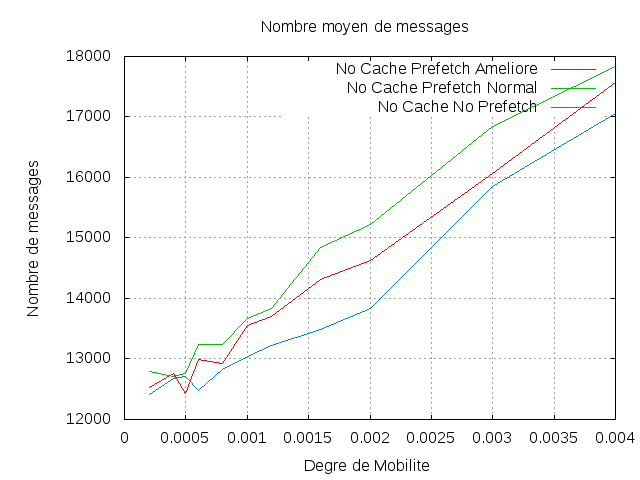
\includegraphics[scale=0.5]{../CacheCode/SolipsisPeersim/resultats/Courbes/Courbes_Final_Rapport/Nombre_Messages_Prefetchs.png}
        \caption{Schéma montrant le nombre de messages}
        \label{courbeNbMessPrefetch}
        \end{figure}

\par La solution que nous avons mis en place permet d'avoir une meilleure cohérence de la topologie. Certains nœuds, qui était pris et qui se révélaient être inutiles, ne sont plus préchargés. Le nombre de nœuds qui est dans la zone de connaissance d'une autre nœuds mais pas dans sa liste des voisins, augmentent logiquement avec le degré de mobilité. Ce nombre augmente car les mouvements sont en hausse et il y a donc de plus en plus de changements dans la liste des voisins à faire, et les différents délais des messages ou des mécanismes sont limitant pour conserver une bonne topologie. L'introduction du préchargement améliore aussi sensiblement la règle de l'enveloppe connexe de Solipsis.

	\begin{figure}[!h]
        \centering
        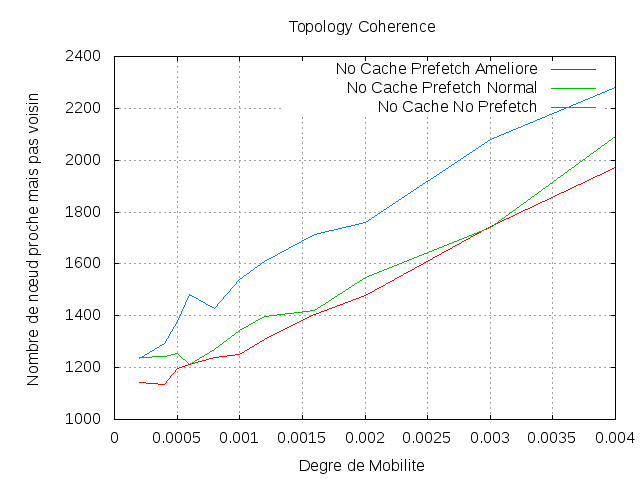
\includegraphics[scale=0.5]{../CacheCode/SolipsisPeersim/resultats/Courbes/Courbes_Final_Rapport/Topology_Coherence_Prefetchs.png}
	\caption{Schéma montrant la cohérence de la topologie}
	\label{courbeTopoPrefetch}
        \end{figure}



\subsection{Conclusion et perspectives}
Le gain sur la cohérence de la topologie de notre solution, est minime mais étant donné qu'il économise en plus des messages, le résultat est donc positif. Le gain sur la topologie pourrait probablement être meilleur si nous regardions encore d'autres paramètres. Mieux regarder les directions, en fonction de la distance des nœuds avec le nœud qui souhaite précharger, pourrait peut être permettre de mieux choisir les nœuds.
Une autre amélioration pourrait être de chercher parmi des nœuds qui peuvent être hors du cône, mais dans un périmètre proche pour ne pas rajouter trop de nœuds à contacter sinon trop de messages seraient alors émis. Si ce mécanisme permet de d'augmenter l'efficacité du préchargement, il peut aussi être possible de regarder avec un angle plus grand de façon périodique.


\newpage
